\chapter{研究方法}
\section{研究設計與流程}

測試文字測試文字測試文字測試文字測試文字測試文字測試文字測試文字測試文字測試文字測試文字測試文字測試文字測試文字測試文字測試文字測試文字測試文字測試文字測試文字測試文字測試文字測試文字測試文字測試文字測試文字測試文字測試文字測試文字測試文字測試文字測試文字測試文字測試文字測試文字測試文字測試文字測試文字測試文字測試文字測試文字測試文字測試文字測試文字測試文字測試文字測試文字測試文字測試文字測試文字測試文字測試文字測試文字測試文字測試文字測試文字測試文字測試文字測試文字測試文字測試文字測試文字測試文字測試文字測試文字測試文字測試文字測試文字測試文字測試文字測試文字測試文字測試文字測試文字測試文字測試文字測試文字測試文字測試文字測試文字測試文字測試文字測試文字測試文字測試文字測試文字測試文字測試文字測試文字測試文字測試文字測試文字測試文字測試文字測試文字測試文字測試文字測試文字測試文字測試文字測試文字測試文字測試文字測試文字測試文字測試文字

測試文字測試文字測試文字測試文字測試文字測試文字測試文字測試文字測試文字測試文字測試文字測試文字測試文字測試文字測試文字測試文字測試文字測試文字測試文字測試文字測試文字測試文字測試文字測試文字測試文字測試文字測試文字測試文字測試文字測試文字測試文字測試文字測試文字測試文字測試文字測試文字測試文字測試文字測試文字測試文字測試文字測試文字測試文字測試文字測試文字測試文字測試文字測試文字測試文字測試文字測試文字測試文字測試文字

圖\ref{i:debug}顯示了遇到機械機構問題時採用的解法流程圖。
\begin{figure}[!htbp]
\centering

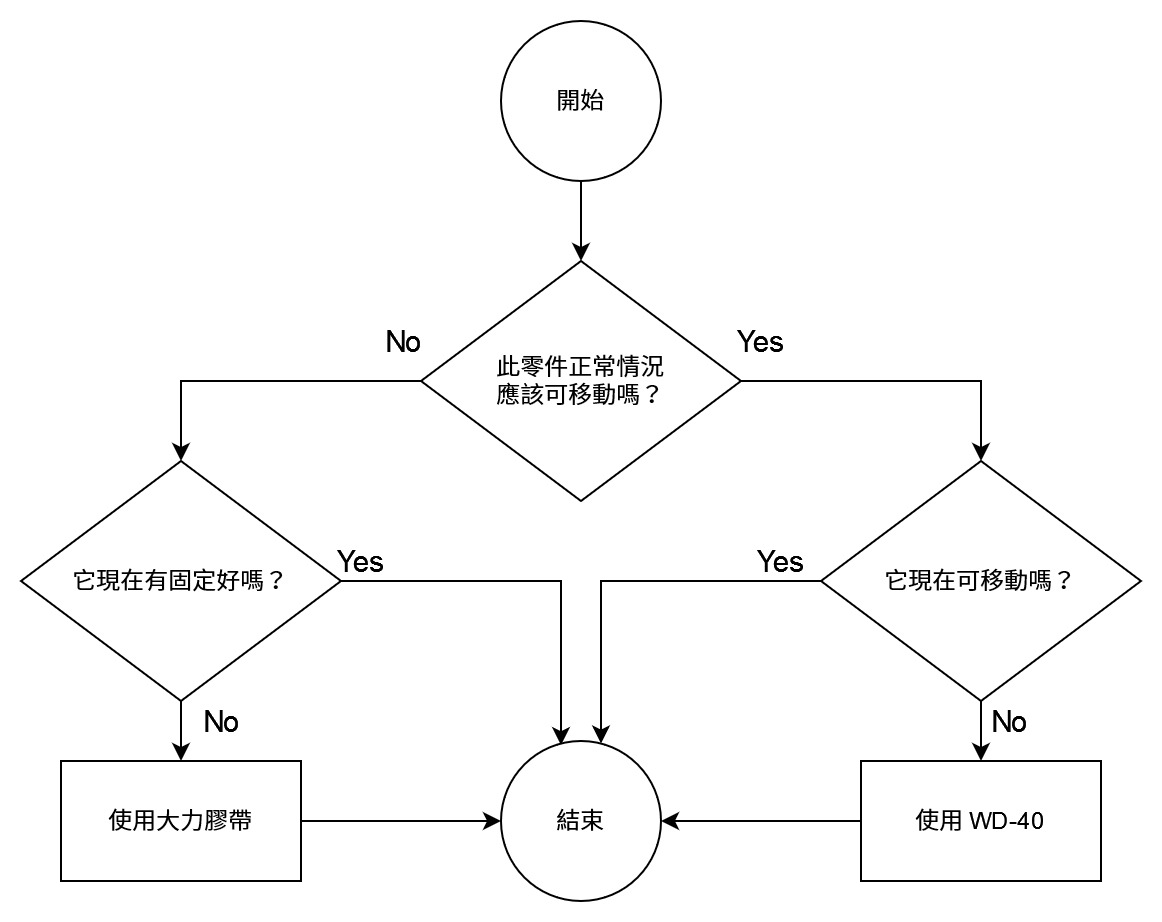
\includegraphics[width=.85\columnwidth]{images/debug.jpg}
\caption{機械問題除錯流程圖}
\label{i:debug}

\end{figure}


樹範例如~\ref{i:tree}
\begin{figure}[!htbp]
\centering

\tikzset{every tree node/.style={align=center},
    level distance=40pt,
    sibling distance=6pt}
\begin{tikzpicture}
\Tree[.root
       [ (a) ]
       [.node
         [.node
           [ (b) ]
           [ (c) ]
         ]
         [.node
           [ (d) ]
           [ (e) ]
           [ (f) ]
           [ (g) ]
           [ (h) ]
         ]
       ]
     ]

\end{tikzpicture}

\caption{A tree. }
\label{i:tree}
\end{figure}


長條圖範例如~\ref{i:barchart}
\input{figures/barchart}

本研究分組如表~\ref{t:group}
\input{tables/group}
